\documentclass[1p]{elsarticle_modified}
%\bibliographystyle{elsarticle-num}

%\usepackage[colorlinks]{hyperref}
%\usepackage{abbrmath_seonhwa} %\Abb, \Ascr, \Acal ,\Abf, \Afrak
\usepackage{amsfonts}
\usepackage{amssymb}
\usepackage{amsmath}
\usepackage{amsthm}
\usepackage{scalefnt}
\usepackage{amsbsy}
\usepackage{kotex}
\usepackage{caption}
\usepackage{subfig}
\usepackage{color}
\usepackage{graphicx}
\usepackage{xcolor} %% white, black, red, green, blue, cyan, magenta, yellow
\usepackage{float}
\usepackage{setspace}
\usepackage{hyperref}

\usepackage{tikz}
\usetikzlibrary{arrows}

\usepackage{multirow}
\usepackage{array} % fixed length table
\usepackage{hhline}

%%%%%%%%%%%%%%%%%%%%%
\makeatletter
\renewcommand*\env@matrix[1][\arraystretch]{%
	\edef\arraystretch{#1}%
	\hskip -\arraycolsep
	\let\@ifnextchar\new@ifnextchar
	\array{*\c@MaxMatrixCols c}}
\makeatother %https://tex.stackexchange.com/questions/14071/how-can-i-increase-the-line-spacing-in-a-matrix
%%%%%%%%%%%%%%%

\usepackage[normalem]{ulem}

\newcommand{\msout}[1]{\ifmmode\text{\sout{\ensuremath{#1}}}\else\sout{#1}\fi}
%SOURCE: \msout is \stkout macro in https://tex.stackexchange.com/questions/20609/strikeout-in-math-mode

\newcommand{\cancel}[1]{
	\ifmmode
	{\color{red}\msout{#1}}
	\else
	{\color{red}\sout{#1}}
	\fi
}

\newcommand{\add}[1]{
	{\color{blue}\uwave{#1}}
}

\newcommand{\replace}[2]{
	\ifmmode
	{\color{red}\msout{#1}}{\color{blue}\uwave{#2}}
	\else
	{\color{red}\sout{#1}}{\color{blue}\uwave{#2}}
	\fi
}

\newcommand{\Sol}{\mathcal{S}} %segment
\newcommand{\D}{D} %diagram
\newcommand{\A}{\mathcal{A}} %arc


%%%%%%%%%%%%%%%%%%%%%%%%%%%%%5 test

\def\sl{\operatorname{\textup{SL}}(2,\Cbb)}
\def\psl{\operatorname{\textup{PSL}}(2,\Cbb)}
\def\quan{\mkern 1mu \triangleright \mkern 1mu}

\theoremstyle{definition}
\newtheorem{thm}{Theorem}[section]
\newtheorem{prop}[thm]{Proposition}
\newtheorem{lem}[thm]{Lemma}
\newtheorem{ques}[thm]{Question}
\newtheorem{cor}[thm]{Corollary}
\newtheorem{defn}[thm]{Definition}
\newtheorem{exam}[thm]{Example}
\newtheorem{rmk}[thm]{Remark}
\newtheorem{alg}[thm]{Algorithm}

\newcommand{\I}{\sqrt{-1}}
\begin{document}

%\begin{frontmatter}
%
%\title{Boundary parabolic representations of knots up to 8 crossings}
%
%%% Group authors per affiliation:
%\author{Yunhi Cho} 
%\address{Department of Mathematics, University of Seoul, Seoul, Korea}
%\ead{yhcho@uos.ac.kr}
%
%
%\author{Seonhwa Kim} %\fnref{s_kim}}
%\address{Center for Geometry and Physics, Institute for Basic Science, Pohang, 37673, Korea}
%\ead{ryeona17@ibs.re.kr}
%
%\author{Hyuk Kim}
%\address{Department of Mathematical Sciences, Seoul National University, Seoul 08826, Korea}
%\ead{hyukkim@snu.ac.kr}
%
%\author{Seokbeom Yoon}
%\address{Department of Mathematical Sciences, Seoul National University, Seoul, 08826,  Korea}
%\ead{sbyoon15@snu.ac.kr}
%
%\begin{abstract}
%We find all boundary parabolic representation of knots up to 8 crossings.
%
%\end{abstract}
%\begin{keyword}
%    \MSC[2010] 57M25 
%\end{keyword}
%
%\end{frontmatter}

%\linenumbers
%\tableofcontents
%
\newcommand\colored[1]{\textcolor{white}{\rule[-0.35ex]{0.8em}{1.4ex}}\kern-0.8em\color{red} #1}%
%\newcommand\colored[1]{\textcolor{white}{ #1}\kern-2.17ex	\textcolor{white}{ #1}\kern-1.81ex	\textcolor{white}{ #1}\kern-2.15ex\color{red}#1	}

{\Large $\underline{12a_{0202}~(K12a_{0202})}$}

\setlength{\tabcolsep}{10pt}
\renewcommand{\arraystretch}{1.6}
\vspace{1cm}\begin{tabular}{m{100pt}>{\centering\arraybackslash}m{274pt}}
\multirow{5}{120pt}{
	\centering
	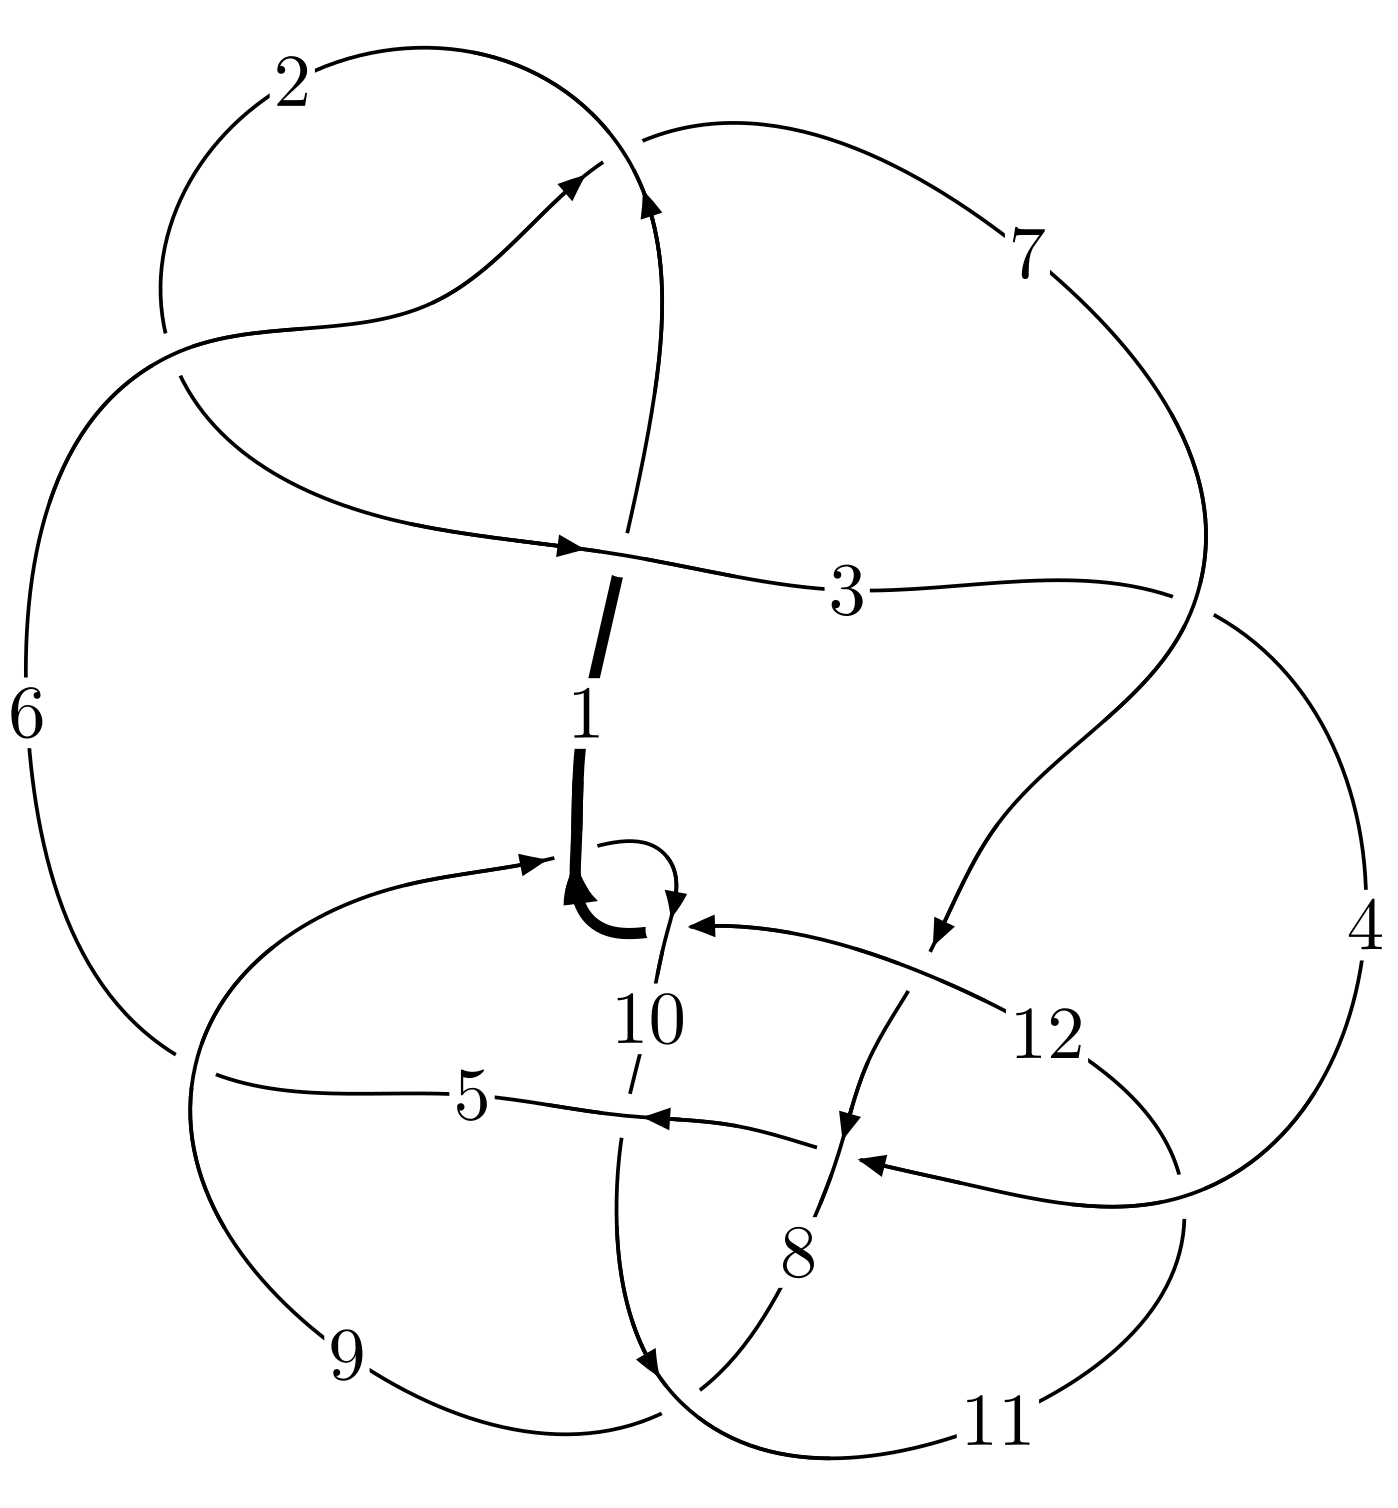
\includegraphics[width=112pt]{../../../GIT/diagram.site/Diagrams/png/1003_12a_0202.png}\\
\ \ \ A knot diagram\footnotemark}&
\allowdisplaybreaks
\textbf{Linearized knot diagam} \\
\cline{2-2}
 &
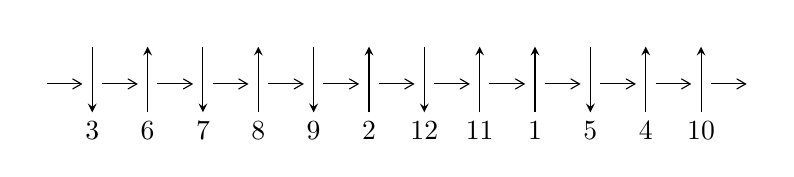
\begin{tikzpicture}[x=20pt, y=17pt]
	% nodes
	\node (C0) at (0, 0) {};
	\node (C1) at (1, 0) {};
	\node (C1U) at (1, +1) {};
	\node (C1D) at (1, -1) {3};

	\node (C2) at (2, 0) {};
	\node (C2U) at (2, +1) {};
	\node (C2D) at (2, -1) {6};

	\node (C3) at (3, 0) {};
	\node (C3U) at (3, +1) {};
	\node (C3D) at (3, -1) {7};

	\node (C4) at (4, 0) {};
	\node (C4U) at (4, +1) {};
	\node (C4D) at (4, -1) {8};

	\node (C5) at (5, 0) {};
	\node (C5U) at (5, +1) {};
	\node (C5D) at (5, -1) {9};

	\node (C6) at (6, 0) {};
	\node (C6U) at (6, +1) {};
	\node (C6D) at (6, -1) {2};

	\node (C7) at (7, 0) {};
	\node (C7U) at (7, +1) {};
	\node (C7D) at (7, -1) {12};

	\node (C8) at (8, 0) {};
	\node (C8U) at (8, +1) {};
	\node (C8D) at (8, -1) {11};

	\node (C9) at (9, 0) {};
	\node (C9U) at (9, +1) {};
	\node (C9D) at (9, -1) {1};

	\node (C10) at (10, 0) {};
	\node (C10U) at (10, +1) {};
	\node (C10D) at (10, -1) {5};

	\node (C11) at (11, 0) {};
	\node (C11U) at (11, +1) {};
	\node (C11D) at (11, -1) {4};

	\node (C12) at (12, 0) {};
	\node (C12U) at (12, +1) {};
	\node (C12D) at (12, -1) {10};
	\node (C13) at (13, 0) {};

	% arrows
	\draw[->,>={angle 60}]
	(C0) edge (C1) (C1) edge (C2) (C2) edge (C3) (C3) edge (C4) (C4) edge (C5) (C5) edge (C6) (C6) edge (C7) (C7) edge (C8) (C8) edge (C9) (C9) edge (C10) (C10) edge (C11) (C11) edge (C12) (C12) edge (C13) ;	\draw[->,>=stealth]
	(C1U) edge (C1D) (C2D) edge (C2U) (C3U) edge (C3D) (C4D) edge (C4U) (C5U) edge (C5D) (C6D) edge (C6U) (C7U) edge (C7D) (C8D) edge (C8U) (C9D) edge (C9U) (C10U) edge (C10D) (C11D) edge (C11U) (C12D) edge (C12U) ;
	\end{tikzpicture} \\
\hhline{~~} \\& 
\textbf{Solving Sequence} \\ \cline{2-2} 
 &
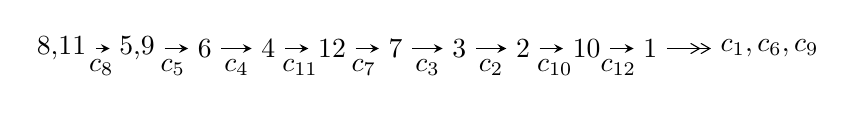
\begin{tikzpicture}[x=23pt, y=7pt]
	% node
	\node (A0) at (-1/8, 0) {8,11};
	\node (A1) at (17/16, 0) {5,9};
	\node (A2) at (17/8, 0) {6};
	\node (A3) at (25/8, 0) {4};
	\node (A4) at (33/8, 0) {12};
	\node (A5) at (41/8, 0) {7};
	\node (A6) at (49/8, 0) {3};
	\node (A7) at (57/8, 0) {2};
	\node (A8) at (65/8, 0) {10};
	\node (A9) at (73/8, 0) {1};
	\node (C1) at (1/2, -1) {$c_{8}$};
	\node (C2) at (13/8, -1) {$c_{5}$};
	\node (C3) at (21/8, -1) {$c_{4}$};
	\node (C4) at (29/8, -1) {$c_{11}$};
	\node (C5) at (37/8, -1) {$c_{7}$};
	\node (C6) at (45/8, -1) {$c_{3}$};
	\node (C7) at (53/8, -1) {$c_{2}$};
	\node (C8) at (61/8, -1) {$c_{10}$};
	\node (C9) at (69/8, -1) {$c_{12}$};
	\node (A10) at (11, 0) {$c_{1},c_{6},c_{9}$};

	% edge
	\draw[->,>=stealth]	
	(A0) edge (A1) (A1) edge (A2) (A2) edge (A3) (A3) edge (A4) (A4) edge (A5) (A5) edge (A6) (A6) edge (A7) (A7) edge (A8) (A8) edge (A9) ;
	\draw[->>,>={angle 60}]	
	(A9) edge (A10);
\end{tikzpicture} \\ 

\end{tabular} \\

\footnotetext{
The image of knot diagram is generated by the software ``\textbf{Draw programme}" developed by Andrew Bartholomew(\url{http://www.layer8.co.uk/maths/draw/index.htm\#Running-draw}), where we modified some parts for our purpose(\url{https://github.com/CATsTAILs/LinksPainter}).
}\phantom \\ \newline 
\centering \textbf{Ideals for irreducible components\footnotemark of $X_{\text{par}}$} 
 
\begin{align*}
I^u_{1}&=\langle 
-5.85376\times10^{42} u^{30}-4.11584\times10^{43} u^{29}+\cdots+6.43717\times10^{43} b-1.52717\times10^{45},\\
\phantom{I^u_{1}}&\phantom{= \langle  }-1.65310\times10^{43} u^{30}-4.70509\times10^{44} u^{29}+\cdots+4.05542\times10^{45} a-7.34210\times10^{46},\\
\phantom{I^u_{1}}&\phantom{= \langle  }u^{31}+7 u^{30}+\cdots+1062 u+189\rangle \\
\\
I^v_{1}&=\langle 
a,\;b+1,\;v^2+v+1\rangle \\
I^v_{2}&=\langle 
a,\;b^2- b+1,\;v-1\rangle \\
I^v_{3}&=\langle 
a,\;4 v^3- v^2+5 b+22 v-2,\;v^4- v^3+6 v^2-4 v+1\rangle \\
\end{align*}
\raggedright * 4 irreducible components of $\dim_{\mathbb{C}}=0$, with total 39 representations.\\
\footnotetext{All coefficients of polynomials are rational numbers. But the coefficients are sometimes approximated in decimal forms when there is not enough margin.}
\newpage
\renewcommand{\arraystretch}{1}
\centering \section*{I. $I^u_{1}= \langle -5.85\times10^{42} u^{30}-4.12\times10^{43} u^{29}+\cdots+6.44\times10^{43} b-1.53\times10^{45},\;-1.65\times10^{43} u^{30}-4.71\times10^{44} u^{29}+\cdots+4.06\times10^{45} a-7.34\times10^{46},\;u^{31}+7 u^{30}+\cdots+1062 u+189 \rangle$}
\flushleft \textbf{(i) Arc colorings}\\
\begin{tabular}{m{7pt} m{180pt} m{7pt} m{180pt} }
\flushright $a_{8}=$&$\begin{pmatrix}1\\0\end{pmatrix}$ \\
\flushright $a_{11}=$&$\begin{pmatrix}0\\u\end{pmatrix}$ \\
\flushright $a_{5}=$&$\begin{pmatrix}0.00407627 u^{30}+0.116020 u^{29}+\cdots+71.4362 u+18.1044\\0.0909369 u^{30}+0.639387 u^{29}+\cdots+117.933 u+23.7242\end{pmatrix}$ \\
\flushright $a_{9}=$&$\begin{pmatrix}1\\- u^2\end{pmatrix}$ \\
\flushright $a_{6}=$&$\begin{pmatrix}0.0650669 u^{30}+0.372522 u^{29}+\cdots+47.1836 u+10.9151\\-0.150639 u^{30}-0.814503 u^{29}+\cdots-51.5391 u-8.48759\end{pmatrix}$ \\
\flushright $a_{4}=$&$\begin{pmatrix}-0.0868606 u^{30}-0.523367 u^{29}+\cdots-46.4970 u-5.61977\\0.0909369 u^{30}+0.639387 u^{29}+\cdots+117.933 u+23.7242\end{pmatrix}$ \\
\flushright $a_{12}=$&$\begin{pmatrix}-0.141645 u^{30}-0.885725 u^{29}+\cdots-143.560 u-32.5033\\0.136354 u^{30}+0.848688 u^{29}+\cdots+128.206 u+26.8843\end{pmatrix}$ \\
\flushright $a_{7}=$&$\begin{pmatrix}0.159417 u^{30}+1.05337 u^{29}+\cdots+203.681 u+47.2113\\0.0886170 u^{30}+0.486093 u^{29}+\cdots+27.1810 u+2.41793\end{pmatrix}$ \\
\flushright $a_{3}=$&$\begin{pmatrix}-0.134901 u^{30}-0.754733 u^{29}+\cdots-92.6270 u-19.9654\\-0.0991047 u^{30}-0.789918 u^{29}+\cdots-201.805 u-46.7404\end{pmatrix}$ \\
\flushright $a_{2}=$&$\begin{pmatrix}0.0568952 u^{30}+0.361874 u^{29}+\cdots+34.6334 u+5.22896\\-0.426439 u^{30}-2.74939 u^{29}+\cdots-446.153 u-94.9907\end{pmatrix}$ \\
\flushright $a_{10}=$&$\begin{pmatrix}0.000387022 u^{30}-0.0156505 u^{29}+\cdots-26.4970 u-7.97560\\0.00567803 u^{30}+0.0213866 u^{29}+\cdots-9.14249 u-2.35655\end{pmatrix}$ \\
\flushright $a_{1}=$&$\begin{pmatrix}-0.123885 u^{30}-0.755730 u^{29}+\cdots-104.552 u-23.7852\\0.109341 u^{30}+0.684999 u^{29}+\cdots+104.246 u+21.1806\end{pmatrix}$\\&\end{tabular}
\flushleft \textbf{(ii) Obstruction class $= 1$}\\~\\
\flushleft \textbf{(iii) Cusp Shapes $= 0.415132 u^{30}+2.95762 u^{29}+\cdots+715.270 u+178.126$}\\~\\
\newpage\renewcommand{\arraystretch}{1}
\flushleft \textbf{(iv) u-Polynomials at the component}\newline \\
\begin{tabular}{m{50pt}|m{274pt}}
Crossings & \hspace{64pt}u-Polynomials at each crossing \\
\hline $$\begin{aligned}c_{1}\end{aligned}$$&$\begin{aligned}
&u^{31}-18 u^{30}+\cdots-10 u+1
\end{aligned}$\\
\hline $$\begin{aligned}c_{2}\end{aligned}$$&$\begin{aligned}
&u^{31}-2 u^{30}+\cdots+4 u-1
\end{aligned}$\\
\hline $$\begin{aligned}c_{3}\end{aligned}$$&$\begin{aligned}
&u^{31}+2 u^{30}+\cdots-14 u^2-1
\end{aligned}$\\
\hline $$\begin{aligned}c_{4}\end{aligned}$$&$\begin{aligned}
&u^{31}-3 u^{30}+\cdots-3 u+1
\end{aligned}$\\
\hline $$\begin{aligned}c_{5}\end{aligned}$$&$\begin{aligned}
&u^{31}+2 u^{30}+\cdots+5 u-1
\end{aligned}$\\
\hline $$\begin{aligned}c_{6}\end{aligned}$$&$\begin{aligned}
&u^{31}+2 u^{30}+\cdots+4 u+1
\end{aligned}$\\
\hline $$\begin{aligned}c_{7}\end{aligned}$$&$\begin{aligned}
&u^{31}+4 u^{30}+\cdots+3 u+1
\end{aligned}$\\
\hline $$\begin{aligned}c_{8}\end{aligned}$$&$\begin{aligned}
&u^{31}+7 u^{30}+\cdots+1062 u+189
\end{aligned}$\\
\hline $$\begin{aligned}c_{9}\end{aligned}$$&$\begin{aligned}
&u^{31}+10 u^{30}+\cdots+3 u+1
\end{aligned}$\\
\hline $$\begin{aligned}c_{10}\end{aligned}$$&$\begin{aligned}
&u^{31}-3 u^{29}+\cdots- u+1
\end{aligned}$\\
\hline $$\begin{aligned}c_{11}\end{aligned}$$&$\begin{aligned}
&u^{31}- u^{30}+\cdots-3 u^2+1
\end{aligned}$\\
\hline $$\begin{aligned}c_{12}\end{aligned}$$&$\begin{aligned}
&u^{31}-10 u^{30}+\cdots+3 u-1
\end{aligned}$\\
\hline
\end{tabular}\\~\\
\newpage\renewcommand{\arraystretch}{1}
\flushleft \textbf{(v) Riley Polynomials at the component}\newline \\
\begin{tabular}{m{50pt}|m{274pt}}
Crossings & \hspace{64pt}Riley Polynomials at each crossing \\
\hline $$\begin{aligned}c_{1}\end{aligned}$$&$\begin{aligned}
&y^{31}-2 y^{30}+\cdots+10 y-1
\end{aligned}$\\
\hline $$\begin{aligned}c_{2},c_{6}\end{aligned}$$&$\begin{aligned}
&y^{31}+18 y^{30}+\cdots-10 y-1
\end{aligned}$\\
\hline $$\begin{aligned}c_{3}\end{aligned}$$&$\begin{aligned}
&y^{31}-10 y^{30}+\cdots-28 y-1
\end{aligned}$\\
\hline $$\begin{aligned}c_{4}\end{aligned}$$&$\begin{aligned}
&y^{31}+3 y^{30}+\cdots+11 y-1
\end{aligned}$\\
\hline $$\begin{aligned}c_{5}\end{aligned}$$&$\begin{aligned}
&y^{31}+10 y^{30}+\cdots-23 y-1
\end{aligned}$\\
\hline $$\begin{aligned}c_{7}\end{aligned}$$&$\begin{aligned}
&y^{31}-26 y^{30}+\cdots-7 y-1
\end{aligned}$\\
\hline $$\begin{aligned}c_{8}\end{aligned}$$&$\begin{aligned}
&y^{31}-17 y^{30}+\cdots-40554 y-35721
\end{aligned}$\\
\hline $$\begin{aligned}c_{9},c_{12}\end{aligned}$$&$\begin{aligned}
&y^{31}+14 y^{30}+\cdots-27 y-1
\end{aligned}$\\
\hline $$\begin{aligned}c_{10}\end{aligned}$$&$\begin{aligned}
&y^{31}-6 y^{30}+\cdots+13 y-1
\end{aligned}$\\
\hline $$\begin{aligned}c_{11}\end{aligned}$$&$\begin{aligned}
&y^{31}-13 y^{30}+\cdots+6 y-1
\end{aligned}$\\
\hline
\end{tabular}\\~\\
\newpage\flushleft \textbf{(vi) Complex Volumes and Cusp Shapes}
$$\begin{array}{c|c|c}  
\text{Solutions to }I^u_{1}& \I (\text{vol} + \sqrt{-1}CS) & \text{Cusp shape}\\
 \hline 
\begin{aligned}
u &= -0.787754 + 0.671220 I \\
a &= \phantom{-}0.071441 - 0.869841 I \\
b &= \phantom{-}1.11016 - 1.12553 I\end{aligned}
 & \phantom{-}0.66300 - 4.58967 I & \phantom{-}3.64967 + 6.32585 I \\ \hline\begin{aligned}
u &= -0.787754 - 0.671220 I \\
a &= \phantom{-}0.071441 + 0.869841 I \\
b &= \phantom{-}1.11016 + 1.12553 I\end{aligned}
 & \phantom{-}0.66300 + 4.58967 I & \phantom{-}3.64967 - 6.32585 I \\ \hline\begin{aligned}
u &= -0.919933 + 0.149004 I \\
a &= \phantom{-}0.754923 + 0.119454 I \\
b &= -0.731306 - 0.126839 I\end{aligned}
 & \phantom{-}0.96861 - 3.12100 I & \phantom{-}7.33060 + 2.35538 I \\ \hline\begin{aligned}
u &= -0.919933 - 0.149004 I \\
a &= \phantom{-}0.754923 - 0.119454 I \\
b &= -0.731306 + 0.126839 I\end{aligned}
 & \phantom{-}0.96861 + 3.12100 I & \phantom{-}7.33060 - 2.35538 I \\ \hline\begin{aligned}
u &= -0.882506 + 0.604366 I \\
a &= \phantom{-}0.000444 + 0.754013 I \\
b &= -1.08064 + 1.17241 I\end{aligned}
 & -1.31127 - 9.18738 I & \phantom{-}2.03905 + 12.84834 I \\ \hline\begin{aligned}
u &= -0.882506 - 0.604366 I \\
a &= \phantom{-}0.000444 - 0.754013 I \\
b &= -1.08064 - 1.17241 I\end{aligned}
 & -1.31127 + 9.18738 I & \phantom{-}2.03905 - 12.84834 I \\ \hline\begin{aligned}
u &= \phantom{-}1.085000 + 0.299590 I \\
a &= -0.718094 + 0.604115 I \\
b &= \phantom{-}0.112159 + 0.738606 I\end{aligned}
 & -3.66102 + 5.86923 I & -0.31180 - 5.53881 I \\ \hline\begin{aligned}
u &= \phantom{-}1.085000 - 0.299590 I \\
a &= -0.718094 - 0.604115 I \\
b &= \phantom{-}0.112159 - 0.738606 I\end{aligned}
 & -3.66102 - 5.86923 I & -0.31180 + 5.53881 I \\ \hline\begin{aligned}
u &= -0.289850 + 0.728639 I \\
a &= \phantom{-}0.48734 - 1.87783 I \\
b &= \phantom{-}1.19769 - 1.43281 I\end{aligned}
 & \phantom{-}0.27311 - 2.22846 I & \phantom{-}7.52450 + 10.82880 I \\ \hline\begin{aligned}
u &= -0.289850 - 0.728639 I \\
a &= \phantom{-}0.48734 + 1.87783 I \\
b &= \phantom{-}1.19769 + 1.43281 I\end{aligned}
 & \phantom{-}0.27311 + 2.22846 I & \phantom{-}7.52450 - 10.82880 I\\
 \hline 
 \end{array}$$\newpage$$\begin{array}{c|c|c}  
\text{Solutions to }I^u_{1}& \I (\text{vol} + \sqrt{-1}CS) & \text{Cusp shape}\\
 \hline 
\begin{aligned}
u &= -1.208330 + 0.213280 I \\
a &= -0.563685 - 0.106371 I \\
b &= \phantom{-}0.578875 + 0.081419 I\end{aligned}
 & \phantom{-}2.49777 + 0.42674 I & \phantom{-}3.8814 - 13.6068 I \\ \hline\begin{aligned}
u &= -1.208330 - 0.213280 I \\
a &= -0.563685 + 0.106371 I \\
b &= \phantom{-}0.578875 - 0.081419 I\end{aligned}
 & \phantom{-}2.49777 - 0.42674 I & \phantom{-}3.8814 + 13.6068 I \\ \hline\begin{aligned}
u &= -1.004870 + 0.756525 I \\
a &= -0.138979 + 0.649444 I \\
b &= -0.97827 + 1.09815 I\end{aligned}
 & -2.54917 - 2.29555 I & \phantom{-}2.17391 + 2.92369 I \\ \hline\begin{aligned}
u &= -1.004870 - 0.756525 I \\
a &= -0.138979 - 0.649444 I \\
b &= -0.97827 - 1.09815 I\end{aligned}
 & -2.54917 + 2.29555 I & \phantom{-}2.17391 - 2.92369 I \\ \hline\begin{aligned}
u &= \phantom{-}1.261950 + 0.109878 I \\
a &= \phantom{-}0.676138 - 0.385755 I \\
b &= -0.077347 - 0.656336 I\end{aligned}
 & -6.52646 + 10.71380 I & -3.90729 - 8.40713 I \\ \hline\begin{aligned}
u &= \phantom{-}1.261950 - 0.109878 I \\
a &= \phantom{-}0.676138 + 0.385755 I \\
b &= -0.077347 + 0.656336 I\end{aligned}
 & -6.52646 - 10.71380 I & -3.90729 + 8.40713 I \\ \hline\begin{aligned}
u &= -0.425245 + 1.202740 I \\
a &= -0.989675 + 0.636178 I \\
b &= -1.50889 + 0.69268 I\end{aligned}
 & -5.08590 - 6.12096 I & -10.22352 + 5.74476 I \\ \hline\begin{aligned}
u &= -0.425245 - 1.202740 I \\
a &= -0.989675 - 0.636178 I \\
b &= -1.50889 - 0.69268 I\end{aligned}
 & -5.08590 + 6.12096 I & -10.22352 - 5.74476 I \\ \hline\begin{aligned}
u &= -0.941908 + 0.964204 I \\
a &= \phantom{-}0.302323 - 0.638136 I \\
b &= \phantom{-}1.014340 - 0.955285 I\end{aligned}
 & -0.97627 - 4.81638 I & \phantom{-}1.86561 + 11.56814 I \\ \hline\begin{aligned}
u &= -0.941908 - 0.964204 I \\
a &= \phantom{-}0.302323 + 0.638136 I \\
b &= \phantom{-}1.014340 + 0.955285 I\end{aligned}
 & -0.97627 + 4.81638 I & \phantom{-}1.86561 - 11.56814 I\\
 \hline 
 \end{array}$$\newpage$$\begin{array}{c|c|c}  
\text{Solutions to }I^u_{1}& \I (\text{vol} + \sqrt{-1}CS) & \text{Cusp shape}\\
 \hline 
\begin{aligned}
u &= \phantom{-}0.103232 + 0.545002 I \\
a &= -0.56419 + 2.65696 I \\
b &= -0.36747 + 1.47669 I\end{aligned}
 & -0.74907 + 3.79069 I & \phantom{-}6.38246 - 10.09885 I \\ \hline\begin{aligned}
u &= \phantom{-}0.103232 - 0.545002 I \\
a &= -0.56419 - 2.65696 I \\
b &= -0.36747 - 1.47669 I\end{aligned}
 & -0.74907 - 3.79069 I & \phantom{-}6.38246 + 10.09885 I \\ \hline\begin{aligned}
u &= \phantom{-}0.60387 + 1.31633 I \\
a &= -0.369398 - 0.916044 I \\
b &= -0.826490 - 0.760871 I\end{aligned}
 & -6.87994 + 5.02111 I & -5.16614 - 5.44554 I \\ \hline\begin{aligned}
u &= \phantom{-}0.60387 - 1.31633 I \\
a &= -0.369398 + 0.916044 I \\
b &= -0.826490 + 0.760871 I\end{aligned}
 & -6.87994 - 5.02111 I & -5.16614 + 5.44554 I \\ \hline\begin{aligned}
u &= \phantom{-}1.38864 + 0.56571 I \\
a &= \phantom{-}0.414352 - 0.550377 I \\
b &= -0.223840 - 0.647984 I\end{aligned}
 & -7.66190 + 2.29159 I & -5.67077 - 3.09442 I \\ \hline\begin{aligned}
u &= \phantom{-}1.38864 - 0.56571 I \\
a &= \phantom{-}0.414352 + 0.550377 I \\
b &= -0.223840 + 0.647984 I\end{aligned}
 & -7.66190 - 2.29159 I & -5.67077 + 3.09442 I \\ \hline\begin{aligned}
u &= -1.60304\phantom{ +0.000000I} \\
a &= -0.427829\phantom{ +0.000000I} \\
b &= \phantom{-}0.481754\phantom{ +0.000000I}\end{aligned}
 & \phantom{-}1.81126\phantom{ +0.000000I} & -9.27850\phantom{ +0.000000I} \\ \hline\begin{aligned}
u &= \phantom{-}1.12150 + 1.17887 I \\
a &= -0.044962 + 0.711521 I \\
b &= \phantom{-}0.481462 + 0.651796 I\end{aligned}
 & -4.85303 + 3.78421 I & -1.98912 - 7.10308 I \\ \hline\begin{aligned}
u &= \phantom{-}1.12150 - 1.17887 I \\
a &= -0.044962 - 0.711521 I \\
b &= \phantom{-}0.481462 - 0.651796 I\end{aligned}
 & -4.85303 - 3.78421 I & -1.98912 + 7.10308 I \\ \hline\begin{aligned}
u &= -1.80227 + 0.16548 I \\
a &= \phantom{-}0.372128 + 0.038139 I \\
b &= -0.441313 - 0.027890 I\end{aligned}
 & -1.24263 + 4.03762 I & -10.43934 + 0. I\phantom{ +0.000000I}\\
 \hline 
 \end{array}$$\newpage$$\begin{array}{c|c|c}  
\text{Solutions to }I^u_{1}& \I (\text{vol} + \sqrt{-1}CS) & \text{Cusp shape}\\
 \hline 
\begin{aligned}
u &= -1.80227 - 0.16548 I \\
a &= \phantom{-}0.372128 - 0.038139 I \\
b &= -0.441313 + 0.027890 I\end{aligned}
 & -1.24263 - 4.03762 I & -10.43934 + 0. I\phantom{ +0.000000I}\\
 \hline 
 \end{array}$$\newpage\newpage\renewcommand{\arraystretch}{1}
\centering \section*{II. $I^v_{1}= \langle a,\;b+1,\;v^2+v+1 \rangle$}
\flushleft \textbf{(i) Arc colorings}\\
\begin{tabular}{m{7pt} m{180pt} m{7pt} m{180pt} }
\flushright $a_{8}=$&$\begin{pmatrix}1\\0\end{pmatrix}$ \\
\flushright $a_{11}=$&$\begin{pmatrix}v\\0\end{pmatrix}$ \\
\flushright $a_{5}=$&$\begin{pmatrix}0\\-1\end{pmatrix}$ \\
\flushright $a_{9}=$&$\begin{pmatrix}1\\0\end{pmatrix}$ \\
\flushright $a_{6}=$&$\begin{pmatrix}1\\-1\end{pmatrix}$ \\
\flushright $a_{4}=$&$\begin{pmatrix}1\\-1\end{pmatrix}$ \\
\flushright $a_{12}=$&$\begin{pmatrix}2 v\\- v\end{pmatrix}$ \\
\flushright $a_{7}=$&$\begin{pmatrix}-2 v-1\\v+1\end{pmatrix}$ \\
\flushright $a_{3}=$&$\begin{pmatrix}v+3\\-2\end{pmatrix}$ \\
\flushright $a_{2}=$&$\begin{pmatrix}2\\v-1\end{pmatrix}$ \\
\flushright $a_{10}=$&$\begin{pmatrix}v\\- v\end{pmatrix}$ \\
\flushright $a_{1}=$&$\begin{pmatrix}2 v+1\\- v-1\end{pmatrix}$\\&\end{tabular}
\flushleft \textbf{(ii) Obstruction class $= 1$}\\~\\
\flushleft \textbf{(iii) Cusp Shapes $= -8 v-1$}\\~\\
\newpage\renewcommand{\arraystretch}{1}
\flushleft \textbf{(iv) u-Polynomials at the component}\newline \\
\begin{tabular}{m{50pt}|m{274pt}}
Crossings & \hspace{64pt}u-Polynomials at each crossing \\
\hline $$\begin{aligned}c_{1},c_{3},c_{6}\\c_{7},c_{10},c_{11}\\c_{12}\end{aligned}$$&$\begin{aligned}
&u^2- u+1
\end{aligned}$\\
\hline $$\begin{aligned}c_{2},c_{9}\end{aligned}$$&$\begin{aligned}
&u^2+u+1
\end{aligned}$\\
\hline $$\begin{aligned}c_{4},c_{5}\end{aligned}$$&$\begin{aligned}
&(u-1)^2
\end{aligned}$\\
\hline $$\begin{aligned}c_{8}\end{aligned}$$&$\begin{aligned}
&u^2
\end{aligned}$\\
\hline
\end{tabular}\\~\\
\newpage\renewcommand{\arraystretch}{1}
\flushleft \textbf{(v) Riley Polynomials at the component}\newline \\
\begin{tabular}{m{50pt}|m{274pt}}
Crossings & \hspace{64pt}Riley Polynomials at each crossing \\
\hline $$\begin{aligned}c_{1},c_{2},c_{3}\\c_{6},c_{7},c_{9}\\c_{10},c_{11},c_{12}\end{aligned}$$&$\begin{aligned}
&y^2+y+1
\end{aligned}$\\
\hline $$\begin{aligned}c_{4},c_{5}\end{aligned}$$&$\begin{aligned}
&(y-1)^2
\end{aligned}$\\
\hline $$\begin{aligned}c_{8}\end{aligned}$$&$\begin{aligned}
&y^2
\end{aligned}$\\
\hline
\end{tabular}\\~\\
\newpage\flushleft \textbf{(vi) Complex Volumes and Cusp Shapes}
$$\begin{array}{c|c|c}  
\text{Solutions to }I^v_{1}& \I (\text{vol} + \sqrt{-1}CS) & \text{Cusp shape}\\
 \hline 
\begin{aligned}
v &= -0.500000 + 0.866025 I \\
a &= \phantom{-0.000000 } 0 \\
b &= -1.00000\phantom{ +0.000000I}\end{aligned}
 & \phantom{-0.000000 -}4.05977 I & \phantom{-}3.00000 - 6.92820 I \\ \hline\begin{aligned}
v &= -0.500000 - 0.866025 I \\
a &= \phantom{-0.000000 } 0 \\
b &= -1.00000\phantom{ +0.000000I}\end{aligned}
 & \phantom{-0.000000 } -4.05977 I & \phantom{-}3.00000 + 6.92820 I\\
 \hline 
 \end{array}$$\newpage\newpage\renewcommand{\arraystretch}{1}
\centering \section*{III. $I^v_{2}= \langle a,\;b^2- b+1,\;v-1 \rangle$}
\flushleft \textbf{(i) Arc colorings}\\
\begin{tabular}{m{7pt} m{180pt} m{7pt} m{180pt} }
\flushright $a_{8}=$&$\begin{pmatrix}1\\0\end{pmatrix}$ \\
\flushright $a_{11}=$&$\begin{pmatrix}1\\0\end{pmatrix}$ \\
\flushright $a_{5}=$&$\begin{pmatrix}0\\b\end{pmatrix}$ \\
\flushright $a_{9}=$&$\begin{pmatrix}1\\0\end{pmatrix}$ \\
\flushright $a_{6}=$&$\begin{pmatrix}- b\\b\end{pmatrix}$ \\
\flushright $a_{4}=$&$\begin{pmatrix}- b\\b\end{pmatrix}$ \\
\flushright $a_{12}=$&$\begin{pmatrix}b\\- b+1\end{pmatrix}$ \\
\flushright $a_{7}=$&$\begin{pmatrix}0\\b\end{pmatrix}$ \\
\flushright $a_{3}=$&$\begin{pmatrix}- b\\b-1\end{pmatrix}$ \\
\flushright $a_{2}=$&$\begin{pmatrix}-1\\0\end{pmatrix}$ \\
\flushright $a_{10}=$&$\begin{pmatrix}1\\- b+1\end{pmatrix}$ \\
\flushright $a_{1}=$&$\begin{pmatrix}0\\- b\end{pmatrix}$\\&\end{tabular}
\flushleft \textbf{(ii) Obstruction class $= 1$}\\~\\
\flushleft \textbf{(iii) Cusp Shapes $= -8 b+4$}\\~\\
\newpage\renewcommand{\arraystretch}{1}
\flushleft \textbf{(iv) u-Polynomials at the component}\newline \\
\begin{tabular}{m{50pt}|m{274pt}}
Crossings & \hspace{64pt}u-Polynomials at each crossing \\
\hline $$\begin{aligned}c_{1},c_{3},c_{6}\\c_{7},c_{10},c_{11}\\c_{12}\end{aligned}$$&$\begin{aligned}
&u^2- u+1
\end{aligned}$\\
\hline $$\begin{aligned}c_{2},c_{4},c_{5}\\c_{9}\end{aligned}$$&$\begin{aligned}
&u^2+u+1
\end{aligned}$\\
\hline $$\begin{aligned}c_{8}\end{aligned}$$&$\begin{aligned}
&u^2
\end{aligned}$\\
\hline
\end{tabular}\\~\\
\newpage\renewcommand{\arraystretch}{1}
\flushleft \textbf{(v) Riley Polynomials at the component}\newline \\
\begin{tabular}{m{50pt}|m{274pt}}
Crossings & \hspace{64pt}Riley Polynomials at each crossing \\
\hline $$\begin{aligned}c_{1},c_{2},c_{3}\\c_{4},c_{5},c_{6}\\c_{7},c_{9},c_{10}\\c_{11},c_{12}\end{aligned}$$&$\begin{aligned}
&y^2+y+1
\end{aligned}$\\
\hline $$\begin{aligned}c_{8}\end{aligned}$$&$\begin{aligned}
&y^2
\end{aligned}$\\
\hline
\end{tabular}\\~\\
\newpage\flushleft \textbf{(vi) Complex Volumes and Cusp Shapes}
$$\begin{array}{c|c|c}  
\text{Solutions to }I^v_{2}& \I (\text{vol} + \sqrt{-1}CS) & \text{Cusp shape}\\
 \hline 
\begin{aligned}
v &= \phantom{-}1.00000\phantom{ +0.000000I} \\
a &= \phantom{-0.000000 } 0 \\
b &= \phantom{-}0.500000 + 0.866025 I\end{aligned}
 & \phantom{-0.000000 -}4.05977 I & \phantom{-0.000000 } 0. - 6.92820 I \\ \hline\begin{aligned}
v &= \phantom{-}1.00000\phantom{ +0.000000I} \\
a &= \phantom{-0.000000 } 0 \\
b &= \phantom{-}0.500000 - 0.866025 I\end{aligned}
 & \phantom{-0.000000 } -4.05977 I & \phantom{-0.000000 -}0. + 6.92820 I\\
 \hline 
 \end{array}$$\newpage\newpage\renewcommand{\arraystretch}{1}
\centering \section*{IV. $I^v_{3}= \langle a,\;4 v^3- v^2+5 b+22 v-2,\;v^4- v^3+6 v^2-4 v+1 \rangle$}
\flushleft \textbf{(i) Arc colorings}\\
\begin{tabular}{m{7pt} m{180pt} m{7pt} m{180pt} }
\flushright $a_{8}=$&$\begin{pmatrix}1\\0\end{pmatrix}$ \\
\flushright $a_{11}=$&$\begin{pmatrix}v\\0\end{pmatrix}$ \\
\flushright $a_{5}=$&$\begin{pmatrix}0\\-\frac{4}{5} v^3+\frac{1}{5} v^2-\frac{22}{5} v+\frac{2}{5}\end{pmatrix}$ \\
\flushright $a_{9}=$&$\begin{pmatrix}1\\0\end{pmatrix}$ \\
\flushright $a_{6}=$&$\begin{pmatrix}\frac{4}{5} v^3-\frac{1}{5} v^2+\frac{22}{5} v-\frac{2}{5}\\-\frac{4}{5} v^3+\frac{1}{5} v^2-\frac{22}{5} v+\frac{2}{5}\end{pmatrix}$ \\
\flushright $a_{4}=$&$\begin{pmatrix}\frac{4}{5} v^3-\frac{1}{5} v^2+\frac{22}{5} v-\frac{2}{5}\\-\frac{4}{5} v^3+\frac{1}{5} v^2-\frac{22}{5} v+\frac{2}{5}\end{pmatrix}$ \\
\flushright $a_{12}=$&$\begin{pmatrix}\frac{3}{5} v^3-\frac{2}{5} v^2+\frac{24}{5} v-\frac{9}{5}\\-\frac{3}{5} v^3+\frac{2}{5} v^2-\frac{19}{5} v+\frac{9}{5}\end{pmatrix}$ \\
\flushright $a_{7}=$&$\begin{pmatrix}-\frac{2}{5} v^3+\frac{3}{5} v^2-\frac{16}{5} v+\frac{6}{5}\\\frac{3}{5} v^3-\frac{2}{5} v^2+\frac{19}{5} v-\frac{4}{5}\end{pmatrix}$ \\
\flushright $a_{3}=$&$\begin{pmatrix}\frac{4}{5} v^3-\frac{1}{5} v^2+\frac{27}{5} v-\frac{7}{5}\\-\frac{7}{5} v^3+\frac{3}{5} v^2-\frac{41}{5} v+\frac{11}{5}\end{pmatrix}$ \\
\flushright $a_{2}=$&$\begin{pmatrix}\frac{6}{5} v^3-\frac{4}{5} v^2+\frac{38}{5} v-\frac{18}{5}\\-\frac{9}{5} v^3+\frac{6}{5} v^2-\frac{52}{5} v+\frac{22}{5}\end{pmatrix}$ \\
\flushright $a_{10}=$&$\begin{pmatrix}v\\-\frac{3}{5} v^3+\frac{2}{5} v^2-\frac{19}{5} v+\frac{9}{5}\end{pmatrix}$ \\
\flushright $a_{1}=$&$\begin{pmatrix}\frac{2}{5} v^3-\frac{3}{5} v^2+\frac{16}{5} v-\frac{6}{5}\\-\frac{3}{5} v^3+\frac{2}{5} v^2-\frac{19}{5} v+\frac{4}{5}\end{pmatrix}$\\&\end{tabular}
\flushleft \textbf{(ii) Obstruction class $= 1$}\\~\\
\flushleft \textbf{(iii) Cusp Shapes $= 4 v^3-4 v^2+23 v-8$}\\~\\
\newpage\renewcommand{\arraystretch}{1}
\flushleft \textbf{(iv) u-Polynomials at the component}\newline \\
\begin{tabular}{m{50pt}|m{274pt}}
Crossings & \hspace{64pt}u-Polynomials at each crossing \\
\hline $$\begin{aligned}c_{1},c_{3},c_{6}\\c_{7},c_{12}\end{aligned}$$&$\begin{aligned}
&(u^2- u+1)^2
\end{aligned}$\\
\hline $$\begin{aligned}c_{2},c_{9}\end{aligned}$$&$\begin{aligned}
&(u^2+u+1)^2
\end{aligned}$\\
\hline $$\begin{aligned}c_{4},c_{5}\end{aligned}$$&$\begin{aligned}
&u^4- u^3+2 u+1
\end{aligned}$\\
\hline $$\begin{aligned}c_{8}\end{aligned}$$&$\begin{aligned}
&u^4
\end{aligned}$\\
\hline $$\begin{aligned}c_{10},c_{11}\end{aligned}$$&$\begin{aligned}
&u^4+u^3+3 u^2+u+1
\end{aligned}$\\
\hline
\end{tabular}\\~\\
\newpage\renewcommand{\arraystretch}{1}
\flushleft \textbf{(v) Riley Polynomials at the component}\newline \\
\begin{tabular}{m{50pt}|m{274pt}}
Crossings & \hspace{64pt}Riley Polynomials at each crossing \\
\hline $$\begin{aligned}c_{1},c_{2},c_{3}\\c_{6},c_{7},c_{9}\\c_{12}\end{aligned}$$&$\begin{aligned}
&(y^2+y+1)^2
\end{aligned}$\\
\hline $$\begin{aligned}c_{4},c_{5}\end{aligned}$$&$\begin{aligned}
&y^4- y^3+6 y^2-4 y+1
\end{aligned}$\\
\hline $$\begin{aligned}c_{8}\end{aligned}$$&$\begin{aligned}
&y^4
\end{aligned}$\\
\hline $$\begin{aligned}c_{10},c_{11}\end{aligned}$$&$\begin{aligned}
&y^4+5 y^3+9 y^2+5 y+1
\end{aligned}$\\
\hline
\end{tabular}\\~\\
\newpage\flushleft \textbf{(vi) Complex Volumes and Cusp Shapes}
$$\begin{array}{c|c|c}  
\text{Solutions to }I^v_{3}& \I (\text{vol} + \sqrt{-1}CS) & \text{Cusp shape}\\
 \hline 
\begin{aligned}
v &= \phantom{-}0.351597 + 0.233523 I \\
a &= \phantom{-0.000000 } 0 \\
b &= -1.12196 - 1.05376 I\end{aligned}
 & \phantom{-0.000000 } 0 & -0.24584 + 5.00967 I \\ \hline\begin{aligned}
v &= \phantom{-}0.351597 - 0.233523 I \\
a &= \phantom{-0.000000 } 0 \\
b &= -1.12196 + 1.05376 I\end{aligned}
 & \phantom{-0.000000 } 0 & -0.24584 - 5.00967 I \\ \hline\begin{aligned}
v &= \phantom{-}0.14840 + 2.36455 I \\
a &= \phantom{-0.000000 } 0 \\
b &= \phantom{-}0.621964 + 0.187730 I\end{aligned}
 & \phantom{-0.000000 } 0 & \phantom{-}7.74584 - 0.67954 I \\ \hline\begin{aligned}
v &= \phantom{-}0.14840 - 2.36455 I \\
a &= \phantom{-0.000000 } 0 \\
b &= \phantom{-}0.621964 - 0.187730 I\end{aligned}
 & \phantom{-0.000000 } 0 & \phantom{-}7.74584 + 0.67954 I\\
 \hline 
 \end{array}$$\newpage
\newpage\renewcommand{\arraystretch}{1}
\centering \section*{ V. u-Polynomials}
\begin{tabular}{m{50pt}|m{274pt}}
Crossings & \hspace{64pt}u-Polynomials at each crossing \\
\hline $$\begin{aligned}c_{1}\end{aligned}$$&$\begin{aligned}
&((u^2- u+1)^4)(u^{31}-18 u^{30}+\cdots-10 u+1)
\end{aligned}$\\
\hline $$\begin{aligned}c_{2}\end{aligned}$$&$\begin{aligned}
&((u^2+u+1)^4)(u^{31}-2 u^{30}+\cdots+4 u-1)
\end{aligned}$\\
\hline $$\begin{aligned}c_{3}\end{aligned}$$&$\begin{aligned}
&((u^2- u+1)^4)(u^{31}+2 u^{30}+\cdots-14 u^2-1)
\end{aligned}$\\
\hline $$\begin{aligned}c_{4}\end{aligned}$$&$\begin{aligned}
&((u-1)^2)(u^2+u+1)(u^4- u^3+2 u+1)(u^{31}-3 u^{30}+\cdots-3 u+1)
\end{aligned}$\\
\hline $$\begin{aligned}c_{5}\end{aligned}$$&$\begin{aligned}
&((u-1)^2)(u^2+u+1)(u^4- u^3+2 u+1)(u^{31}+2 u^{30}+\cdots+5 u-1)
\end{aligned}$\\
\hline $$\begin{aligned}c_{6}\end{aligned}$$&$\begin{aligned}
&((u^2- u+1)^4)(u^{31}+2 u^{30}+\cdots+4 u+1)
\end{aligned}$\\
\hline $$\begin{aligned}c_{7}\end{aligned}$$&$\begin{aligned}
&((u^2- u+1)^4)(u^{31}+4 u^{30}+\cdots+3 u+1)
\end{aligned}$\\
\hline $$\begin{aligned}c_{8}\end{aligned}$$&$\begin{aligned}
&u^8(u^{31}+7 u^{30}+\cdots+1062 u+189)
\end{aligned}$\\
\hline $$\begin{aligned}c_{9}\end{aligned}$$&$\begin{aligned}
&((u^2+u+1)^4)(u^{31}+10 u^{30}+\cdots+3 u+1)
\end{aligned}$\\
\hline $$\begin{aligned}c_{10}\end{aligned}$$&$\begin{aligned}
&((u^2- u+1)^2)(u^4+u^3+3 u^2+u+1)(u^{31}-3 u^{29}+\cdots- u+1)
\end{aligned}$\\
\hline $$\begin{aligned}c_{11}\end{aligned}$$&$\begin{aligned}
&((u^2- u+1)^2)(u^4+u^3+3 u^2+u+1)(u^{31}- u^{30}+\cdots-3 u^2+1)
\end{aligned}$\\
\hline $$\begin{aligned}c_{12}\end{aligned}$$&$\begin{aligned}
&((u^2- u+1)^4)(u^{31}-10 u^{30}+\cdots+3 u-1)
\end{aligned}$\\
\hline
\end{tabular}\newpage\renewcommand{\arraystretch}{1}
\centering \section*{ VI. Riley Polynomials}
\begin{tabular}{m{50pt}|m{274pt}}
Crossings & \hspace{64pt}Riley Polynomials at each crossing \\
\hline $$\begin{aligned}c_{1}\end{aligned}$$&$\begin{aligned}
&((y^2+y+1)^4)(y^{31}-2 y^{30}+\cdots+10 y-1)
\end{aligned}$\\
\hline $$\begin{aligned}c_{2},c_{6}\end{aligned}$$&$\begin{aligned}
&((y^2+y+1)^4)(y^{31}+18 y^{30}+\cdots-10 y-1)
\end{aligned}$\\
\hline $$\begin{aligned}c_{3}\end{aligned}$$&$\begin{aligned}
&((y^2+y+1)^4)(y^{31}-10 y^{30}+\cdots-28 y-1)
\end{aligned}$\\
\hline $$\begin{aligned}c_{4}\end{aligned}$$&$\begin{aligned}
&((y-1)^2)(y^2+y+1)(y^4- y^3+\cdots-4 y+1)(y^{31}+3 y^{30}+\cdots+11 y-1)
\end{aligned}$\\
\hline $$\begin{aligned}c_{5}\end{aligned}$$&$\begin{aligned}
&((y-1)^2)(y^2+y+1)(y^4- y^3+\cdots-4 y+1)(y^{31}+10 y^{30}+\cdots-23 y-1)
\end{aligned}$\\
\hline $$\begin{aligned}c_{7}\end{aligned}$$&$\begin{aligned}
&((y^2+y+1)^4)(y^{31}-26 y^{30}+\cdots-7 y-1)
\end{aligned}$\\
\hline $$\begin{aligned}c_{8}\end{aligned}$$&$\begin{aligned}
&y^8(y^{31}-17 y^{30}+\cdots-40554 y-35721)
\end{aligned}$\\
\hline $$\begin{aligned}c_{9},c_{12}\end{aligned}$$&$\begin{aligned}
&((y^2+y+1)^4)(y^{31}+14 y^{30}+\cdots-27 y-1)
\end{aligned}$\\
\hline $$\begin{aligned}c_{10}\end{aligned}$$&$\begin{aligned}
&((y^2+y+1)^2)(y^4+5 y^3+\cdots+5 y+1)(y^{31}-6 y^{30}+\cdots+13 y-1)
\end{aligned}$\\
\hline $$\begin{aligned}c_{11}\end{aligned}$$&$\begin{aligned}
&((y^2+y+1)^2)(y^4+5 y^3+\cdots+5 y+1)(y^{31}-13 y^{30}+\cdots+6 y-1)
\end{aligned}$\\
\hline
\end{tabular}
\vskip 2pc
\end{document}